\justify
\section{Decisi�n de la carrera que se escogi�}

\justify
La octava pregunta ten�a como prop�sito averiguar si los estudiantes fueron los responsables de escoger la carrera que estudian actualmente. Como se observa en la figura O.2, solo una peque�a parte de la muestra no escogi� su carrera.\\


\begin{figure}[h]
	\begin{center}
		\caption{Proporci�n de  los estudiantes dependiendo de si tuvo oportunidad para escoger su carrera.}
		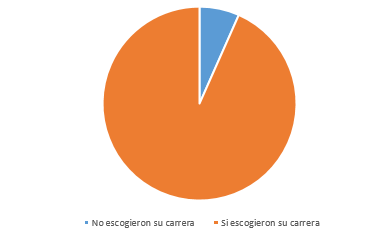
\includegraphics[scale=1]{eleccion-carrera}
	\end{center}
\end{figure}
\bigskip
Al realizar una estimaci�n de la proporci�n poblacional de los valores anteriores, se encuentra que entre el 91\% y 95.8\% de los estudiantes de la Universidad del Valle de Guatemala escogieron su carrera universitaria. Lo que nos indica que los casos en los que los estudiantes fueron obligados a estudiar una determinada carrera son pocos. Por lo cual, si la mayor�a de los estudiantes no siguieron su carrera tentativa fue por decisi�n de ellos.\\

\begin{table}[h]
	\begin{center}
		\caption{Intervalo de confianza al 95\% de la proporci�n poblacional de los estudiantes que escogieron su carrera universitaria.}
		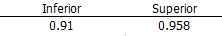
\includegraphics[scale=1]{escogieron-carrera}
	\end{center}
\end{table}




